%
%   This file is part of the APS files in the REVTeX 4 distribution.
%   Version 4.0 of REVTeX, August 2001
%
%   Copyright (c) 2001 The American Physical Society.
%
%   See the REVTeX 4 README file for restrictions and more information.
%
% TeX'ing this file requires that you have AMS-LaTeX 2.0 installed
% as well as the rest of the prerequisites for REVTeX 4.0
%
% See the REVTeX 4 README file
% It also requires running BibTeX. The commands are as follows:
%
%  1)  latex apssamp.tex
%  2)  bibtex apssamp
%  3)  latex apssamp.tex
%  4)  latex apssamp.tex
%
%\documentclass[prb,aps,nobibnotes,twocolumn,doublespace,twocolumngrid,superbib]{revtex4}
%%\documentclass[twocolumn,showpacs,preprintnumbers,amsmath,amssymb]{revtex4}
%\documentclass[preprint,showpacs,preprintnumbers,amsmath,amssymb]{revtex4}

% Some other (several out of many) possibilities
%\documentclass[preprint,aps]{revtex4}
%\documentclass[preprint,aps,draft]{revtex4}
%\documentclass[prb]{revtex4}% Physical Review B

%%\usepackage{amsmath}
%%\usepackage{amssymb}
%%\usepackage{graphicx}% Include figure files
%%\usepackage{dcolumn}% Align table columns on decimal point
%%\usepackage{bm}% bold math

%\documentclass[pre,aps,twocolumn,showpacs,twocolumngrid,superbib]{revtex4}
%\documentclass[prl,aps,twocolumn,showkeys,twocolumngrid,superbib]{revtex4}
%\documentclass[twocolumn,showkeys,showpacs,preprintnumbers,amsmath,amssymb]{revtex4}
\documentclass[prl,twocolumn,showpacs,twocolumngrid,superbib]{revtex4}
%\documentclass[showpacs,preprint,superbib]{revtex4}

\usepackage{graphicx}
\usepackage{amsfonts}
\usepackage{amsmath}
\usepackage{bm}
\usepackage{alltt}
\usepackage{fancyhdr}
\usepackage{dcolumn} 

\pagestyle{fancy}


\def\Tr{{\rm Tr}}
%\nofiles

\begin{document}

%\preprint{APS/123-QED}

%\title{Exact Hartree-Fock exchange gradient and stress within the $\Gamma$-point approximation}
\title{Exchange energy gradients with respect to atomic positions and cell parameters
  within the Hartree-Fock $\Gamma$-point approximation}

\author{Val\'ery Weber}
\email{valery.weber@unifr.ch}
\affiliation{Department of Chemistry, University of Fribourg, 1700 Fribourg, Switzerland.}%
\author{Matt Challacombe}%
\affiliation{Los Alamos National Laboratory, Theoretical Division, Los Alamos 87545, New Mexico, USA.}%

\date{\today}% It is always \today, today,
             %  but any date may be explicitly specified

\begin{abstract}
  Recently, construction of the periodic exact Hartree-Fock exchange 
  [J. Chem. Phys. {\bf ???}, ???, (200?)]
  matrix within the $\Gamma$-point approximation
  has been introduced. In this article, the formalism for the evaluation of 
  the analytical exact Hartree-Fock exchange energy gradients and lattice gradients at 
  the $\Gamma$-point approximation is presented. While the evaluation of the
  periodic exchange energy gradients are similar to their gas phase limit, the exchange
  energy lattice gradients require the accumulation of the gradients acting on atoms multiplied 
  by some appropriate factors and a modified electron repulsion integral (ERI). The latter
  integral arises from the use of the minimal image convention~(MIC). We demonstrate how
  this new ERI can be computed with the help of a modified vertical 
  recurrence relation (VRR) in the frame of the Obara-Saika and Head-Gordon-Pople 
  algorithm.  As an illustration, the analytical gradients and lattice gradients have been used 
  in conjunction with the QUICCA algorithm [K. N\'emeth and M. Challacombe,
  J. Chem. Phys. {\bf 121}, 2877, (2004)] to optimize few periodic 
  systems at the Hartree-Fock level of theory.
\end{abstract}

%\pacs{Valid PACS appear here}% PACS, the Physics and Astronomy
                             % Classification Scheme.
\keywords{Periodic boundary condition, exact Hartree-Fock exchange, atomic gradients, 
lattice gradients.}
                              %display desired
\maketitle

\section{Introduction}

In preceding papers, we have developed linear scaling quantum chemical methods
for construction of the periodic Coulomb, exchange-correlation~\cite{CTymczak04a}
and the exact Hartree-Fock exchange~\cite{CTymczak04b} 
matrices within the $\Gamma$-point approximation. 
In this paper, the implementation of the exact Hartree-Fock exchange
gradients and lattice gradients at the $\Gamma$-point is presented. 
The formalism for the evaluation of the Coulomb and 
exchange-correlation energy cell gradients will be presented 
in a companion paper~\cite{CTymczak05}.

The Hartree-Fock approximation is often a fast, first approximation and 
also a starting point for correlated wavefunction methods.
Also the hybrid Hartree-Fock/Density Functional Theory (HF/DFT) model chemistries
are an important next step in accuracy beyond the Generalized Gradient 
Approximation~\cite{Gill92,Becke93,VBarone96,CAdamo99}. Together with linear
scaling methods for computing the density matrix~\cite{ANiklasson02A,ANiklasson03}, these
advances provide a framework for the application of both HF and HF/DFT 
models to large condensed phase systems, surfaces and wires.

While the $\Gamma$-point approximation uses only the $\mathbf{k}=0$ point to sample
the Brillouin zone, it does however converge to the 
${\bf k}$-space integration in the worst case proportionally to the inverse of the volume of 
the unit cell (See for example Refs.~\cite{CKittel71,NAshcroft76}).
The convergence of the $\Gamma$-point approximation to 
the corresponding ${\bf k}$-space limit was recently 
demonstrated for DFT~\cite{CTymczak04a}, HF and hybrid 
HF/DFT~\cite{CTymczak04b} level of theories.

The $\Gamma$-point approach opens the capabilities of studying very large 
complex and disordered systems such as liquides,....

Finding crystal structures of condensed systems can
be formulated as an identification of the total energy minima
as a function of atomic coordinates and unit-cell vectors.
The problem is then the minimization of the total energy in $M$ dimensions, where
$M=3N+3$. $N$ is the number of atoms, $3N-3$ is the number
of independent coordinates after the elimination of the translation, 
and the number of independent unit-vector elements
after the elimination of unit-cell rotations is 6.
%Gradients and lattice gradients are important concepts in characterizing the states of condensed
%matter. The simulation of system with periodic boundary condition (PBC) 
%involves the atomic positions in the unit cell and the lattice parameters. 
%The location of an energy minimum requires an optimization of both sets 
%of coordinates. 
This minimization can be achieved with the help of an efficient optimizer~\cite{KNemeth04,KNemeth05}
and the knowledge of the periodic energy gradients and cell gradients. 
%The latter represents the derivative of the energy of the unit cell 
%with respect to the unit-cell vectors. 
                                  
The first implementation of the Hartree-Fock cell gradients based on 
Gaussian type atomic orbital (GTAO),
were for one dimensional periodic systems~\cite{HTeramae83,HTeramae84}. 
Other groups have also described such implementation for 
one~\cite{DJacquemin99A,DJacquemin99B} or two~\cite{MTobita03} dimensions. 
The analytical lattice gradient method of density functional theory using GTAO for 
1D extended systems was implemented by Hirata and Iwata~\cite{SHirata98}.
The three dimensional case has been implemented by Kudin and Scuseria 
~\cite{KKudin00A,KKudin00B}. Their approach for the Coulomb problem is 
based on the direct space fast multipole method.
We can also mention the plane-wave local density functional (LDF) formulation
by Nielsen and Martin~\cite{ONielsen85} and the LDF-LCAO derivation of 
the cell gradients by Feibelman~\cite{PFeibelman91}.
Recently Doll, Dovesi and Orlando~\cite{KDoll04} presented 
the implementation of the Hartree-Fock cell gradients into 
the {\sc Crystal03}~\cite{RDovesi00} package for three dimensional systems. 
Their code is based on GTAO and the summation 
of the Coulomb energy is performed with the Ewald method~\cite{PEwald21}, 
which is a combination of direct and reciprocal lattice summations.
For an efficient truncation of the three infinite summations of the exchange
series, the {\sc Crystal03} program uses in the first hand, the decay between local basis function 
products and in the second, the fact that the element of the density 
matrix of an insulator decays exponentially with the distance between 
the two centers.
The strategy to compute the analytical Hartree-Fock gradients for 
periodic system, in the frame of the {\sc Crystal03} package has been 
presented by Doll, Saunders and Harrison~\cite{KDoll01}.
Their implementation is based on the Hermite Gaussian-type function
in the context of the McMurchie-Davidson algorithm~\cite{LMcmurchie78}.


The HF-MIC model is a translationally invariant definition of $\Gamma$-point Hartree-Fock exchange, 
which correctly approaches the k-space integration value in the limit of a
large cell. This is accomplished through introducing a 
minimum image convention (MIC) into the exchange kernel
at the level of primitive two-electron integrals.

As it will be shown latter, the evaluation of the exchange energy gradients,
within the $\Gamma$-point approximation,
does not lead to special difficulties. The implementation requires the evaluation
of the derivative of the ERI's with respect to atomic positions and, 
except the MIC applied at the primitive level, is
similar to what have been done in the past for molecular calculations 
~\cite{SObara86,MGordon88,KIshida91,THelgaker92,KIshida93}.
Difficulties arise when the derivative of the ERI's is taken with respect to lattice 
parameters. In this case the derivative provides, after some manipulations, 
a new type of integral which
arises due to the use of the MIC in our $\Gamma$-point approximation. This integral 
can be evaluated with the help of a modified recurrence relation (RR) similar to the
vertical recurrence relation (VRR) introduced by Obara and Saika~\cite{SObara86}.

The remainder of this paper is organized as follows:
In Section~\ref{Sec:Formalism}, we introduce the formalism and discuss
the implementation of the exact Hartree-Fock exchange energy gradients and cell gradients 
at the $\Gamma$-point approximation. Full optimization of few periodic systems are given
in Section~\ref{Sec:NumExamples} as an illustration of the formalism.
Finally in Section~\ref{Sec:Conclusions} we summarize our results.


\section{Hartree-Fock exchange energy}\label{Sec:Formalism}
The primitive cell is given by the three vectors $\mathbf{a}$, 
$\mathbf{b}$ and $\mathbf{c}$, $M$ is the $3\times3$ matrix composed 
of the primitive lattice vectors
\begin{equation}
  M=(\mathbf{a},\mathbf{b},\mathbf{c}).
\end{equation}
The position of a lattice is $\mathbf{R(n)}=M\mathbf{n}$,
with $\mathbf{n}=(n_a,n_b,n_c)$ a vector of integers.
The position of atom $A$ in the cell $\mathbf{R(n)}$ is $\mathbf{A}=M(\mathbf{f}_A+\mathbf{n})$,
with $\mathbf{f}_A=(f_{Aa},f_{Ab},f_{Ac})$ the fractional coordinates of 
the atom $A$ in the central cell. 
In the following, we will refer to the full set of
fractional coordinates of the atoms in the working cell 
$\mathbf{f}_A,\mathbf{f}_B,\ldots$ as $\{\mathbf{f}_G\}$.

An unnormalized Cartesian Gaussian-type function (CGTF) centered on atom $A$ is
\begin{equation}
  \phi_a(\mathbf{r})=(x-A_x)^{a_x}(y-A_y)^{a_y}(z-A_z)^{a_z}e^{-\zeta_a(\mathbf{r-A})^2},
\end{equation}
where the triad $a=(a_x,a_y,a_z)$ sets the angular symmetry and the exponent $\zeta_a$
is chosen to describe a particular length scale. Gaussian basis functions are often
contracted to approximate atomic eigenfunctions.

%The Hartree-Fock exchange energy is given by
%\begin{equation}
% E^x(\{\mathbf{f}_A\},M)=\Tr(PK)
%\end{equation}
%where $P=P(\{\mathbf{f}_A\},M)$ is the converged density matrix and $K=K(\{\mathbf{f}_A\},M)$ is
%the Hartree-Fock exchange matrix within 
%the MIC $\Gamma$-point approximation~\cite{CTymczak04b}
%and its elements are
%\begin{equation}
%  K_{ab}(\{\mathbf{f}_A\},M)= -\frac{1}{2}\sum_{\substack{\mathbf{m}\mathbf{n}\\c d}}
%  P_{cd}(ac^\mathbf{m}|bd^\mathbf{n})
%\end{equation}
%where the pair of indices $\mathbf{m}$ and $\mathbf{n}$ run over the direct lattice vectors, 
%$c$ and $d$ over the basis functions, $P_{cd}$ is an element of the density matrix 
%and the ERIs are written in the chemist notation.

The Hartree-Fock exchange energy within the MIC $\Gamma$-point approximation~\cite{CTymczak04b} 
is given by
\begin{equation}
 E^x(\{\mathbf{f}_G\},M)=
 -\frac{1}{2}\sum_{\substack{\mathbf{m}\mathbf{n}\\a b c d}}P_{ab}P_{cd}
 (ac^\mathbf{m}|bd^\mathbf{n})
\end{equation}
where the indices $\mathbf{mn}$ run over the direct lattice vectors, 
$abcd$ over the basis functions, $P=P(\{\mathbf{f}_G\},M)$ is the density matrix 
and the ERIs are written in the chemist notation.
%\begin{equation}
%  \begin{split}
%    (ac^\mathbf{m}|bd^\mathbf{n})=
%                    &\iint\phi_a(\mathbf{r}_1)\phi_c(\mathbf{r}_1-M\mathbf{m})\frac{1}{r_{12}}\\
%                    &\times\phi_b(\mathbf{r}_2)\phi_d(\mathbf{r}_2-M\mathbf{n})d^3r_1d^3r_2.
%  \end{split}
%\end{equation}

The minimal image convention is applied in the so-called $K^4$ loop 
(where $K$ is the degree of contraction)
to the interaction vector $\mathbf{P-Q}$ during the evaluation of the ERIs and is 
repeated here for convenience 
\begin{equation}\label{Eq:MIC}
  \mathbf{PQ}=M(\mathbf{f}_{PQ}-[\mathbf{f}_{PQ}-\varepsilon \mathrm{sgn}(\mathbf{f}_{PQ})]),
\end{equation}
where $\mathbf{f}_{PQ}=M^{-1}(\mathbf{P-Q})$, 
$\mathbf{P}=(\zeta_a\mathbf{A}+\zeta_c\mathbf{C})/(\zeta_a+\zeta_c)$, 
$\mathbf{Q}=(\zeta_b\mathbf{B}+\zeta_d\mathbf{D})/(\zeta_b+\zeta_d)$, 
$\varepsilon\approx 10^{-15}$ is 
required to yield a consistent wrapping when distributions lie at the cell boundary 
and $[\bullet]$ is the nearest integer function defined as 
$[x]:=n$ with $x\in \mathbb{R}$, $n\in \mathbb{Z}$ and $|x-n|<1/2$.
Note the $\mathbf{PQ}=\mathbf{P-Q}$ if and only if $[\mathbf{f}_{PQ}-\varepsilon\mathrm{sgn}(\mathbf{f}_{PQ})]$ cancel.
As an example, the MIC-integral over $s$-type functions is given by
\begin{equation}
  \begin{split}
  (00|00)^{(m)}&=\left(\frac{\rho}{\pi}\right)^{\frac{1}{2}}
    \left(\frac{\pi}{\zeta}\right)^{\frac{3}{2}}\left(\frac{\pi}{\eta}\right)^{\frac{3}{2}}\\
    &\times\exp\left(-\frac{\zeta_a\zeta_c}{\zeta}AC^2\right) \\
    &\times\exp\left(-\frac{\zeta_b\zeta_d}{\eta}BD^2\right) \\
    &\times F_{m}(\rho PQ^2)
  \end{split}
\end{equation}
where $\zeta=\zeta_a+\zeta_c$, $\eta=\zeta_b+\zeta_d$, $\rho=\zeta\eta/(\zeta+\eta)$,
$AC^2=|\mathbf{A-C}|^2$, $BD^2=|\mathbf{B-D}|^2$, $PQ^2=|\mathbf{PQ}|^2$ 
is given by Eq.~\ref{Eq:MIC}, $m\in\mathbb{Z}^*$ plays %is a nonnegative integer which
the same role as in the OS algorithm (the integrals with $m=0$ are true ERIs, while
integrals with $m>0$ are auxiliary integrals)
and $F_m(x)=\int_0^1t^{2m}\exp(-xt^2)dt$ is a reduced form of the incomplete gamma function~\cite{IShavitt63}.


\subsection{Gradients}
The exchange energy gradient with respect to the fractional coordinate 
$f_{Gj}$ can be obtained through the linear transform 
\begin{equation*}
 \frac{\partial E^x}{\partial f_{Gj}}\bigg|_P=\sum_{i=x,y,z}M_{ij}\frac{\partial E^x}{\partial G_i}\bigg|_P,
\end{equation*}
where $\partial E^x/\partial G_i|_P$ is the exchange energy gradient wrt atomic position and
is given by
\begin{equation}\label{Eq:Grad}
  \frac{\partial E^x}{\partial G_i}\bigg|_P =
  -\frac{1}{2}\sum_{\substack{\mathbf{m}\mathbf{n}\\a b c d}}P_{ab}P_{cd}
  \frac{\partial(ac^\mathbf{m}|bd^\mathbf{n})}{\partial G_i},
\end{equation}
%\end{eqnarray}
where the indices $abcd$ and $\mathbf{mn}$ run over the basis functions and the
Bravais vectors respectively.

If we assume {\it e.g.} that $\partial PQ_k/\partial A_i=\delta_{ik}\zeta_a/(\zeta_a+\zeta_c)$
(which is true except at the discontinuity points of the nearest integer function) 
it is then possible to see, after further manipulations, 
that the evaluation of the derivative $\partial(ac^\mathbf{m}|bd^\mathbf{n})/\partial G_i$
is completely similar to its correspondent gas phase
limit (except the application of the MIC Eq.~\ref{Eq:MIC} at the $K^4$ loop). 
Therefore, the evaluation of the exchange energy gradients at the $\Gamma$-point
is standard and do not need to be addressed more 
into detail here. Like in the gas phase calculation, the translational 
invariance~\cite{AKorminicki77} can be also used to reduce the computational labor.

\subsection{Lattice Gradients}
The exchange energy lattice gradients are given by
\begin{equation}\label{Eq:Xstress}
  \frac{\partial E^x}{\partial M_{ij}}\bigg|_P=
  -\frac{1}{2}\sum_{\substack{\mathbf{m}\mathbf{n}\\a b c d}}P_{ab}P_{cd}
  \frac{\partial(ac^\mathbf{m}|bd^\mathbf{n})}{\partial M_{ij}},
\end{equation}
where the summations are the same as in~(\ref{Eq:Grad}).
The derivative of the integrals $(ac^\mathbf{m}|bd^\mathbf{n})$, with respect 
to cell parameters $M_{ij}$, can be further decomposed as
\begin{equation}\label{Eq:DerMij}
  \begin{split}
    \frac{\partial (ac^\mathbf{m}|bd^\mathbf{n})}{\partial M_{ij}}
    &=(f_{Aj}-(f_{Dj}+n_j))\frac{\partial (ac^\mathbf{m}|bd^\mathbf{n})}{\partial A_{i}}\\
    &+(f_{Cj}+m_j-(f_{Dj}+n_j))\frac{\partial (ac^\mathbf{m}|bd^\mathbf{n})}{\partial C_{i}}\\
    &+(f_{Bj}-(f_{Dj}+n_j))\frac{\partial (ac^\mathbf{m}|bd^\mathbf{n})}{\partial B_{i}}\\
    &+[ac^\mathbf{m}|bd^\mathbf{n}]_{ij},
  \end{split}
\end{equation}
{\bf ???ABOVE: SHALL WE USE TRANSLATIONAL INVARIANCE???}\\
%\begin{equation}\label{Eq:DerMij}
%  \begin{split}
%    \frac{\partial (ac^\mathbf{m}|bd^\mathbf{n})}{\partial M_{ij}}
%    &=f_{Aj}\frac{\partial (ac^\mathbf{m}|bd^\mathbf{n})}{\partial A_{i}}
%    +(f_{Cj}+m_j)\frac{\partial (ac^\mathbf{m}|bd^\mathbf{n})}{\partial C_{i}}\\
%    &+f_{Bj}\frac{\partial (ac^\mathbf{m}|bd^\mathbf{n})}{\partial B_{i}}
%    +(f_{Dj}+n_j)\frac{\partial (ac^\mathbf{m}|bd^\mathbf{n})}{\partial D_{i}}\\
%    &+[ac^\mathbf{m}|bd^\mathbf{n}]_{ij},
%  \end{split}
%\end{equation}
where we have used the translational invariance~\cite{AKorminicki77}. 
The integral derivatives $\partial (ac^\mathbf{m}|bd^\mathbf{n})/\partial A_{i}$, 
$\partial (ac^\mathbf{m}|bd^\mathbf{n})/\partial B_{i}$ and 
$\partial (ac^\mathbf{m}|bd^\mathbf{n})/\partial C_{i}$ are the same
as the one used to compute the gradients with respect to atomic positions. The extra term 
$[ac^\mathbf{m}|bd^\mathbf{n}]_{ij}$, which is not present in 
previous derivations~\cite{MTobita03,KKudin00B,KDoll04}, 
has its origin in the derivative of the minimal image convention used in 
our $\Gamma$-point approximation. 
This can be seen by taking the derivative of Eq.~(\ref{Eq:MIC}) with respect to $M_{ij}$ as
\begin{equation*}
  \frac{\partial PQ_k}{\partial M_{ij}}=\delta_{ik}(f_{PQj}-[f_{PQj}-\varepsilon\mathrm{sgn}(f_{PQj})]),
\end{equation*}
while the first right hand term $f_{PQj}$ leads, after rearrangement, 
to a contribution of the weighted gradients, 
the second term $[f_{PQj}-\varepsilon \mathrm{sgn}(f_{PQj})]$
gives extra contributions which can be collected into a new integral, the so-called
$[ac^\mathbf{m}|bd^\mathbf{n}]_{ij}$.

%vw THAT ISN'T THAT FAST, IN FACT IT DECREASES AS 1/PQ.
%It is straightforward to see that this integral tends to vanish when 
%the allowed exchange interaction range becomes smaller than half the system size.
%In other words, there is no need to ``wrap'' around the distance between the two 
%distributions centered on $\mathbf{P}$ and $\mathbf{Q}$, i.e.
%$[f_{PQj}-\varepsilon \mathrm{sgn}(f_{PQj})]$ vanishes.

\subsection{Strategy for the evaluation of $[ac|bd]_{ij}$}
The integral $[ac|bd]_{ij}$ can be divided into a product of a $i$ and $j$ part as
\begin{equation*}
 [ac|bd]_{ij}=2\rho[f_{PQj}-\varepsilon\mathrm{sgn}(f_{PQj}) ][ac|bd]_{i},
\end{equation*}
and $\rho$ is defined below. This separation reduces the computational work
in the $K^4$ loop by a non-negligible factor.
In the following, we present a simple approach for the evaluation of
the integral $[ac|bd]_{ij}$ in the spirit of the Obara-Saika~\cite{SObara86}
and Head-Gordon-Pople~\cite{MGordon88} (OS-HGP) algorithm.
The generation of the two-electron integrals is broken up into two
main steps. First, a set of two-electron integrals $c=d=0$ is generated from the
reduced incomplete gamma function~\cite{IShavitt63} 
by mean of a modified version of the OS VRR. Finally,
the Cartesian powers between orbitals of the same electron are transfered using 
the simple two terms horizontal recurrence relation (HRR)~\cite{MGordon88}.
For the evaluation of the integral $[e0|f0]_{i}=[e0|f0]_{i}^{(0)}$, we have 
derived the six-terms MIC-VRR similar
to the one given by Obara and Saika
\begin{equation}\label{Eq:MIC-VRR}
  \begin{split}
    [a&+1_k0|b0]_{i}^{(m)}=
    PA_k[a0|b0]_{i}^{(m)}
    +\delta_{ik}\frac{1}{2\zeta}(a0|b0)^{(m+1)}\\
    &-\frac{\rho}{\zeta}PQ_k[a0|b0]_{i}^{(m+1)}
    +\frac{b_k}{2(\zeta+\eta)}[a0|b-1_k0]_{i}^{(m+1)}\\
    &+\frac{a_k}{2\zeta}
       \left\{
	 [a-1_k0|b0]_{i}^{(m)}-\frac{\rho}{\zeta}[a-1_k0|b0]_{i}^{(m+1)}
       \right\},
  \end{split}
\end{equation}
%where $\zeta=\zeta_a+\zeta_c$, $\eta=\zeta_b+\zeta_d$, $\rho=\zeta\eta/(\zeta+\eta)$,
where $PA_k=P_k-A_k$, $PQ_k$ is given by~(\ref{Eq:MIC})
%, $m\in\mathbb{N}$ plays 
%the same role as in the OS algorithm (the integrals with $m=0$ are true ERIs, while
%integrals with $m>0$ are auxiliary integrals)
and $a_k$ and $b_k$ are the $k$-th components of the angular 
momentum of $\phi_a$ and $\phi_b$ respectively. 
Similar relations may be written down for incrementing angular momentum 
on any other centers by simple substitutions.
The auxiliary integral, $(a0|b0)^{(m+1)}$, are by product of the OS-HGP scheme during
the evaluation of the gradients $\partial (ac|bd)/\partial G_i$.
The use of the above MIC-VRR requires the explicit evaluation of the auxiliary integral
over $s$ functions $[00|00]_{i}^{(m)}$, which is simply
\begin{equation*}
  \begin{split}
    [00|00]_{i}^{(m)}&=
    PQ_i \left(\frac{\rho}{\pi}\right)^{\frac{1}{2}}
    \left(\frac{\pi}{\zeta}\right)^{\frac{3}{2}}\left(\frac{\pi}{\eta}\right)^{\frac{3}{2}}\\
    &\times\exp\left(-\frac{\zeta_a\zeta_c}{\zeta}AC^2\right) \\
    &\times\exp\left(-\frac{\zeta_b\zeta_d}{\eta}BD^2\right) \\
    &\times F_{m+1}(\rho PQ^2) \\
    &=PQ_i(00|00)^{(m+1)}.
  \end{split}
\end{equation*}
%where $AC^2=|\mathbf{A-C}|^2$, $BD^2=|\mathbf{B-D}|^2$, $PQ^2=|\mathbf{PQ}|^2$ and
%$F_m(x)=\int_0^1t^{2m}\exp(-xt^2)dt$ is a reduced form of the incomplete gamma function.
The horizontal recurrence relation~\cite{MGordon88} can be applied to $[a+c0|b+d0]_{ij}$ to give 
finally the target integral $[ac|bd]_{ij}$.
This RR shifts a unit of angular momentum from the first to the second center, i.e.
\begin{equation}~\label{Eq:HRR}
  [ac+1_k|bd]_{ij}=[a+1_kc|bd]_{ij}+AC_k[ac|bd]_{ij},
\end{equation}
where $AC_k=A_k-C_k$. An important feature of the HRR is that the 
constant in the second right hand term involves only the atomic centers
and can be applied outside the contraction loops (i.e. $K^0$).
As the evaluation of the gradients $\partial (ac|bd)/\partial G_i$ and the integral
$[ac|bd]_{ij}$ share the same incomplete gamma functions 
$F_m(x)$ and some intermediate integrals, it is 
advantageous to combine the two algorithms together.
Let us now summarize the proposed algorithm for evaluating the ERI derivatives
with respect to cell parameters within our $\Gamma$-point approximation.
The $F_m(x)$'s are first evaluated through well known methods~\cite{LMcmurchie78,SObara86},
the OS-VRR and the MIC-VRR Eq.~(\ref{Eq:MIC-VRR}) are used together 
to generate the intermediate integrals $(e0|f0)$ and $[e0|f0]_{ij}$. The
desired ERI's are then computed with the help of the HRR Eq.~(\ref{Eq:HRR}),
accumulated with the weighted gradients Eq.~(\ref{Eq:DerMij}) and digested
with the corresponding density matrix elements Eq.~(\ref{Eq:Xstress}) to
yield, finally, the Hartree-Fock exchange contribution to the lattice gradients.


\section{Numerical Examples}\label{Sec:NumExamples}
All developments were implemented in the MondoSCF~\cite{MondoSCF} suite of
linear scaling quantum chemistry programs. The code was compiled 
using the Portland Group F90 compiler {\tt pgf90} v5.1~\cite{pgf90} 
with the~{\tt -O1} options and with the GNU C compiler {\tt gcc} 
v3.2.2 using the~{\tt -O1} flag.
All calculations were carried out on a 1024-node (2048 processors)
dual P4 LinuxBIOS/BProc cluster connected with Myrinet 2000 running
Red-Hat Linux release~9 (Shrike)~\cite{RedHat90}.

%The code was compiled using
%the NAGWare Fortran 95 compiler {\tt f95} Release 5.0(253)~\cite{nagf95} with the 
%{\tt -O2 -Oassumed=always\_contig -Ounroll=1} options and with 
%the GNU C compiler {\tt gcc} v3.2.3 using the {\tt -O1} flag.
%All calculations were carried out on a AMD Athlon MP 2100+ running 
%RedHat Enterprise Linux WS release 3~\cite{RedHatEnt3}.

The {\tt TIGHT} level of numerical accuracy has been used throughout this work.  
Thresholds that define the {\tt TIGHT} accuracy level include a matrix 
threshold $\tau=10^{-6}$, as well as other numerical thresholds 
detailed in Ref.~\cite{CTymczak04a}, which deliver at least 8 digits of 
relative accuracy in the total energy and 4 digits of absolute accuracy 
{\bf ?? WHY ABSOLUTE ACCURACY ??} in the forces.  

In order to demonstrate the capabilities of our implementation of the
Hartree-Fock exchange energy atomic and lattice gradients, we present in this Section 
full optimization studies of 1D and 3D periodic systems without any lattice 
nor atomic positions symmetry constrain. 
Our first benchmark case is a linear chain of HF molecules, the second is
urea, a purely organic compound. The third benchmark system is MgO. 
These two latter systems have been recently optimized at the Hartree-Fock 
level of theory by Doll, Dovesi and Orlando~\cite{KDoll04}.

Table~\ref{Tab:HF-n} shows the progression of the cell constants $a_0$, bond lengths $d$ and
total energies $E$ computed for linear (HF)$_n$ chains at 
the $\Gamma$-point Hartree-Fock with the split-valence 6-31G basis set. 
Comparisons are made to final cell parameter and bond length values obtained 
with a 32 $k$-points in the first Brillouin zone at the 
RHF/6-31G level of theory~\cite{DJacquemin99B}.

\begin{table}[t]
  \centering
  \caption{\protect
    Progression of the Hartree-Fock $\Gamma$-points cell 
    constant $a_0$, bond length $d$ and total energy $E$ for (HF)$_n$ chains
    using the periodic RHF-MIC/6-31G level of theory and the {\tt TIGHT} threshold.
%    $n$ is the number of HF units in the (super)cell.
    Bond lengths and lattice vectors are in \AA~and energies in atomic unit.
  }\label{Tab:HF-n}
  \begin{tabular}{lrllc}
    \toprule
    & $n$ & $\;\;\;a_0$ & $\quad\; d$ & $E/n$ \\
    \hline
    {\sc MondoSCF}\footnote[1]{$\Gamma$-point.}
    &                1  & 4.5449 & 0.9201 & $-$99.9852789 \\
    &                2  & 2.7960 & 0.9257 & $-$99.9958044 \\
    &                4  & 2.4838 & 0.9440 & $-$100.002065 \\
    &                6  & 2.4746 & 0.9453 & $-$100.002213 \\
    &                8  & 2.4745 & 0.9453 & $-$100.002217 \\
    &               10  & 2.4745 & 0.9453 & $-$100.002217 \\
%########################################################
%# cvs update -D ``2005-04-17 07:37'' Optimizer.F90 InCoords.F90
% Rel error vs 100.002217
%A=[
%#    L/n          L       d              E             E/n             log(RelError)
%1  4.544915   4.544915 0.920090   -99.98527897    -99.98527897     -3.77114673046454
%2  2.796054   5.592108 0.925690  -199.9916088145  -99.995804407250 -4.19297596851948
%3  2.523260   7.569780 0.939533  -300.0037675145 -100.001255838167 -5.01721311122697
%4  2.483856   9.935424 0.943980  -400.0082628497 -100.002065712425 -5.82020636658341
%5  2.475845  12.379225 0.945100  -500.0109786307 -100.002195726140 -6.67216333131582
%6  2.474669  14.848014 0.945275  -600.0132802070 -100.002213367833 -7.43984381891266
%7  2.474571  17.321997 0.945325  -700.0155128320 -100.002216118857 -8.05496323522044
%8  2.474471  19.795768 0.945332  -800.0177424840 -100.002217810500  inf
%9  2.474525  22.270725 0.945332  -900.0199573226 -100.002217480289  inf
%10 2.474580  24.745800 0.945335 -1000.0221719941 -100.002217199410  inf
%]
%########################################################
%# cvs update -D ``2005-04-17 07:37'' Optimizer.F90 InCoords.F90
%Rel error vs A(10,4)! scan with a0=2.474580 d=0.945335
%A=[
%#    L          E                E/n           log(RelError)
%1   2.474580   -99.90931751  -99.909317510000  -3.03200127254986
%2   4.949160  -199.98113057  -99.990565285000  -3.93365946786838 
%3   7.423740  -300.00336359 -100.001121196667  -4.96069929811450 
%4   9.898320  -400.00822751 -100.002056877500  -5.79845547146897 
%5  12.372900  -500.01096966 -100.002193932000  -6.65752772485687 
%6  14.847480  -600.01327381 -100.002212301667  -7.43970442086059 
%7  17.322060  -700.01550758 -100.002215368571  -8.24686414765415 
%8  19.796640  -800.01772666 -100.002215832500  -8.98928577493655 
%9  22.271220  -900.01994330 -100.002215922222  -9.89354713250424 
%10 24.745800 -1000.02215935 -100.002215935000  inf
%]
%
%for i=1:9
% log10( abs(A(i,4)+100.002215935000)/(100.002215935000) )
%end
%########################################################
%# cvs update -D ``2005-04-17 07:37'' Optimizer.F90 InCoords.F90
%# a0=2.474580 d=0.945335-0.01!
%A=[
%#      L           F         CellF        log(AbsError F)   log(AbsError CellF) 
%1   2.474580 0.08285215 0.7105489538E-02  -1.12886841274938  -2.45633101570992
%2   4.949160 0.01585675 0.1336029046E-01  -2.13495350060083  -2.01092472900073
%3   7.423740 0.00508851 0.4565773942E-02  -2.46354130511526  -3.01905637077370
%4   9.898320 0.00785897 0.3773522393E-02  -3.17473620497071  -3.78299460127464
%5  12.372900 0.00841246 0.3634280123E-02  -3.93832138475466  -4.59216707108662
%6  14.847480 0.00850540 0.3613436174E-02  -4.65130580973444  -5.32494893139389
%7  17.322060 0.00852375 0.3609480725E-02  -5.40120949323681  -6.10979142942494
%8  19.796640 0.00852700 0.3608902775E-02  -6.14266750356817  -6.70186770821990
%9  22.271220 0.00852760 0.3608851489E-02  -6.92081875394868  -6.83154966090616
%10 24.745800 0.00852772 0.3608704105E-02   inf                inf
%]
%########################################################
%########################################################
%OLD OLD OLD OLD OLD OLD OLD OLD OLD OLD OLD OLD OLD OLD 
%OLD OLD OLD OLD OLD OLD OLD OLD OLD OLD OLD OLD OLD OLD 
% tight
% n     A            E          dHF      A/n         E/n
%  1  4.546343   -99.98527998 0.92013858 4.546343 - 99.98527998
%  2  5.567563  -199.99150998 0.92564118 2.783782 - 99.99575499
%  4  9.933563  -400.00824496 0.94384341 2.483391 -100.00206124
%  6 14.856340  -600.01326989 0.94518511 2.476056 -100.00221164
%  8 19.797923  -800.01772132 0.94521897 2.474740 -100.00221516
% 10 24.748882 -1000.02215549 0.94525870 2.474888 -100.00221555
% verytight
% n     A            E          dHF        A/n         E/n
%  1  4.800062   -99.98537032 0.92065928 4.800062  -99.98537032
%  2  5.594443  -199.99152268 0.92557846 2.797221  -99.99576134
%  3  7.570315  -300.00374196 0.93943432 2.523438 -100.00124732
%  4  9.936075  -400.00824719 0.94388336 2.484018 -100.00206179
%  5 12.379120  -500.01097031 0.94499867 2.475824 -100.00219406
%  6 14.846526  -600.01327386 0.94519146 2.474421 -100.00221231
%  8 19.792315  -800.01772686 0.94523512 2.474039 -100.00221585
% 10 24.740767 -1000.02215951 0.94523867 2.474076 -100.00221595
%
% tight, scan with a0=2.4748 and d=0.94525
%     L          E             E/n          log(RelError)
%  2.4748   -99.90935332  -99.909353320000 -3.03216869570480
%  4.9496  -199.98115488  -99.990577440000 -3.93411264998574
%  7.4244  -300.00336830 -100.001122766667 -4.96132099181872
%  9.8992  -400.00822872 -100.002057180000 -5.79927126890480
% 12.3740  -500.01096991 -100.002193982000 -6.65843662169074
% 14.8488  -600.01327390 -100.002212316667 -7.44102121067321
% 17.3236  -700.01550761 -100.002215372857 -8.24708358999113
% 19.7984  -800.01772671 -100.002215838750 -8.99892527947439 !<those guys should be removed from graph (tight!) 
% 22.2732  -900.01994328 -100.002215920000 -9.72125606791418 !<
% 24.7480 -1000.02215939 -100.002215939000      0            !<
%
% tight, scan with a0=2.4748 and d=0.94525 and NoMIC!
%    L      log(RelError)
% 2.4748  -3.09668203938085
% 7.4244  -3.71849336661178
%12.3740  -3.95069137577253
%17.3236  -4.10175437495038
%22.2732  -4.21356864999351
%27.2228  -4.30236617020264
%#32.1724  -4.37604364689683
%#37.1220  -4.43898766893123
%#42.0716  -4.49395628689044
%#47.0212  -4.54273877305517
%#51.9708  -4.58659003172900
%#56.9204  -4.62641209977567
%#61.8700  -4.66288870463734
%#66.8196  -4.69653762428042
%#71.7692  -4.72776681446666
%#76.7188  -4.75689721889157
%OLD OLD OLD OLD OLD OLD OLD OLD OLD OLD OLD OLD OLD OLD 
%OLD OLD OLD OLD OLD OLD OLD OLD OLD OLD OLD OLD OLD OLD 
%########################################################
%########################################################
% CRYSTAL03 CRYSTAL03 CRYSTAL03 CRYSTAL03 CRYSTAL03 
%32 k-points
%Default parameters
%2.4782 0.9437  -1.000010656644E+02
%2.4772 0.9434  -1.000010635347E+02
%2.4762 0.9434  -1.000010603549E+02
%2.4752 0.9436  -1.000010569145E+02
%2.4742 0.9436  -1.000010535882E+02
%2.4732 0.9436  -1.000010501302E+02
%
%32 k-points
%TOLDEE 12,TOLINTEG 10 12 10 16 16,TOLSCF 12 12
%2.4782 0.9450  -1.000022048954E+02
%2.4772 0.9450  -1.000022052240E+02
%2.4762 0.9451  -1.000022054153E+02
%2.4752 0.9451  -1.000022054997E+02
%2.4751 0.9451  -1.000022055022E+02 <<<
%2.4750 0.9451  -1.000022055014E+02
%2.4749 0.9454  -1.000022054121E+02
%2.4747 0.9454  -1.000022054489E+02
%2.4742 0.9452  -1.000022054730E+02
%2.4732 0.9452  -1.000022053421E+02
%########################################################
%########################################################
%
    \hline
    {\sc POLOPT}\footnote[2]{32 $k$-points~\cite{DJacquemin99B}.} 
    & 1 & 2.4742 & 0.9452  & $-$\\
    {\sc CRYSTAL03}\footnote[3]{32 $k$-points, ITOL: 10 12 10 16 16 and $\Delta E=10^{-12}$.}
    & 1 & 2.4751 & 0.9451 & $-$100.002205\\
% Seem we cannot show those nice results!
%    {\sc GAUSSIAN03}\footnote[3]{32 $k$-points, {\tt Default}.}
%    & 1 & 2.4738 & 0.9455 & $-$100.002216\\%Default
%    {\sc GAUSSIAN03}\footnote[4]{32 $k$-points, {\tt VeryTight}.}
%    & 1 & 2.4742 & 0.9452 & $-$100.002216\\%VeryTight
    \botrule
  \end{tabular}
\end{table}

To analyse the convergence of the $\Gamma$-point energy to the ${\bf k}$-space limit
we have performed single point calculations for the 
(HF)$_n$ chains with cell parameter $a_0=2.4745$\AA~and bond length $d=0.9453$\AA.
Figure~\ref{Fig:CnvgEnergy} shows the relative error to the ${\bf k}$-space limit
with respect to the unit-cell length with and without the MIC.
The absolute convergences of the atomic and cell forces, where
the bond length has been slight contracted by 0.01\AA~to generate 
non-zero forces, are shown in~Fig.~\ref{Fig:CnvgEnergy}.


\begin{figure}[h]
  \caption{Convergence of the $\Gamma$-point relative energy with and without the MIC to the corresponding 
    ${\bf k}$-space limit for the (HF)$_n$ chains with respect to unit-cell length. The cell parameter 
    $a_0=2.4745$\AA~and bond length $d=0.9453$\AA~were held fixed. 
    {\bf !!MAY BE ADD SOMETHING ABOUT FORCES!!}
    Calculations were performed at the RHF-MIC/6-31G level of theory and the {\tt TIGHT} threshold.}\label{Fig:CnvgEnergy}
%  \resizebox*{3.6in}{!}{\includegraphics[angle=-90.00]{./DATA/HF_Energy_cnvg.ps}}
%  \resizebox*{3.6in}{!}{\includegraphics[angle=-90.00]{./DATA/HF_Energy_Forces_cnvg.ps}}
%  \resizebox*{3.6in}{!}{\includegraphics[angle=-90.00]{./DATA/HF_Energy_Forces_cnvg_2.ps}}
  \resizebox*{3.6in}{!}{\includegraphics[angle=-90.00]{./DATA/HF_Energy_Forces_cnvg_3.ps}}
\end{figure}


We have performed full optimization of three dimensional urea supercells 
without any symmetry constraint on the lattice or the atomic positions.
Table~\ref{Tab:Urea} shows the lattice constants, bond lengths, 
bond angles, dihedral angles and total energies
for (urea)$_n$ supercells at the $\Gamma$-point RHF-MIC/6-21G* level of
theory. The basis set are the same as in Ref~\cite{RDovesi90}.
For the seak of comparison, we have also fully optimized a tetragonal lattice
of urea in the $P\bar{4}2_1m$ space group with the 
{\sc Crystal03}~\cite{Crystal03} package and a $2\times 2\times 2$ $k$-points 
integration grid.

\begin{table}[t]
  \centering
  \caption{\protect
    Progression of the Hartree-Fock $\Gamma$-point cell constants, 
    bond lengths, bond angles, dihedral angles 
    and total energy for (urea)$_n$ using the periodic RHF-MIC/6-21G* level of theory 
    and the {\tt TIGHT} threshold. 
%    $n$ is the number of urea units in the (super)cell.
    Lengths, angles and energies are in \AA ngstr\"oms, degrees and atomic units respectively.
  }\label{Tab:Urea}
  \begin{tabular}{lcccc}
    \toprule
    &\multicolumn{3}{c}{\sc{MondoSCF}\footnote[1]{$\Gamma$-point.}}
    &\multicolumn{1}{c}{\sc{Crystal03}\footnote[2]{$2\times 2\times 2$ $k$-points.}} \\
    \hline
    $n$             & 2 & 16 & 54 & 2 \\
    $a_0$           & & & & 5.524 \\
    $c_0$           & & & & 4.642 \\
    $E/n$           & & & &$-$447.68322 \\
    &\multicolumn{4}{c}{Bond lengths} \\
    C$=$O           & & & & \\
    C$-$N           & & & & \\
    N$-$H$_1$       & & & & \\
    N$-$H$_2$       & & & & \\
    &\multicolumn{4}{c}{Bond angles} \\
    OCN             & & & & \\
    CNH$_1$         & & & & \\
    CNH$_2$         & & & & \\
    &\multicolumn{4}{c}{Dihedral angles} \\
    OCNH$_1$        & & & & \\
    OCNH$_2$        & & & & \\
    NCNH$_1$        & & & & \\
    \botrule
  \end{tabular}
\end{table}

Table~\ref{Tab:MgO} shows the progression of the lattice constants and total energies computed
for various MgO supercells at the $\Gamma$-point RHF-MIC level of theory using
the 8-61G basis set for the magnesium and the 8-51G basis set for the oxygen. 
The basis sets were specially optimized for MgO by 
Caus\`a et al~\cite{CBS:861G:MgO} and were obtained from Ref.~\cite{CrystalLib}.
The primitive cubic cell coordinates used for this system are given in 
Ref.~\cite{PBCCoordinates}.
For comparison, we report the optimized lattice parameter of cubic MgO 
obtained with {\sc Crystal03} and a $8\times 8\times 8$ $k$-points integration grid.
\begin{table}[t]
  \centering
  \caption{\protect
    Progression of the Hartree-Fock $\Gamma$-point cell constant $a_0$
    and total energies $E$ for (MgO)$_n$ using the periodic 
    RHF-MIC/8-61G/8-51G level of theory and the {\tt TIGHT} threshold. 
%    $n$ is the number of MgO units in the (super)cell.
    Lengths and energies are in \AA~and atomic unit respectively.
  }\label{Tab:MgO}
  \begin{tabular}{lrccc}
  \toprule
  & $n$ & $a_0$ & $E/n$ & $f_O$ \\
  \hline
    {\sc MondoSCF}\footnote[1]{$\Gamma$-point.}
    &  4  & 4.365 & $-$274.616533 & 0.488 \\% 4.365-274.616533623575FullOpt 2.131
    & 32  & 4.192 & $-$274.664119 & 0.500 \\% 8.385-274.664118754687FullOpt 2.096
    & 108 & 4.192 & $-$274.664299 & 0.500 \\%12.575-274.664299043364FullOpt 2.096
    %&  4\footnote[2]{Full optimization.}        &4.365&$-$274.616533\\%4.365-274.616533623575FullOpt
    %&  4\footnote[3]{Lattice optimization only.}&4.370&$-$274.615477\\%4.370-274.615477868575LattOpt
    %& 32$^b$                                    &4.192&$-$274.664119\\%8.385-274.664118754687FullOpt
    %& 32$^c$                                    &4.192&$-$274.664119\\%8.384-274.664118815087LattOpt
  \hline
    {\sc Crystal03}\footnote[2]{$8\times 8\times 8$ $k$-points.} 
    &  1 & 4.192 & $-$274.664239 & $1/2$ \\%-274.664239121540
  \botrule
  \end{tabular}
\end{table}
%
%Crystal03 HF/8-61G/8-51G 8x8x8 Default
%4.201 -274.66420524315
%4.200 -274.66420889046
%4.199 -274.66421216488
%4.195 -274.66423302172
%4.194 -274.66423838462
%4.193 -274.66423912154
%4.192 -274.66423942700 <<<
%4.191 -274.66423922829
%4.190 -274.66423867131
%4.185 -274.66423067762
%
%Crystal03 PBExc/8-61G/8-51G 8x8x8 What was that?
%4.190 -275.28462703246
%4.200 -275.28469244414
%4.205 -275.28471839588
%4.210 -275.28473181717 
%4.211 -275.28473298902
%4.212 -275.28473352160 <<<
%4.213 -275.28473330887
%4.214 -275.28473191983
%4.215 -275.28473317201
%4.218 -275.28472993937
%4.220 -275.28472509192
%4.230 -275.28467343664 
%
%MgO PBExc Crystal03 User2.bas 8x8x8 default
%4.200 -275.28468980590
%4.205 -275.28471572672
%4.208 -275.28472235701
%4.210 -275.28472911839
%4.211 -275.28473028612
%4.212 -275.28473081270 <<<
%4.213 -275.28473059552
%4.215 -275.28473044697
%4.250 -275.28445240627
%
%MgO B3LYP Crystal03 User2.bas 8x8x8 default
%4.190 -275.43120191268
%4.200 -275.43122829482
%4.202 -275.43123248175
%4.203 -275.43123398833
%4.204 -275.43123514068 <<<
%4.205 -275.43123509457
%4.210 -275.43123002554
%4.215 -275.43121357505
%4.220 -275.43118801547
%4.250 -275.43082055853
%
%MONDO PBExc User2.bas Tight
%  a0         E            d       f
%4.3307 -1100.9726623928 2.1643  0.49976
%
%
%
%
%MONDO B3LYP User2.bas Tight
%
%
%
%
%
%ICE ICE ICE ICE ICE ICE ICE ICE ICE ICE ICE ICE ICE ICE ICE 
% Ferroelectric ordered ice in Cmc21 setting (from Crystal)
% HF/6-31G**/Tight
%               E            A        C
% 2x2x1 -1216.7333268588 9.253791 7.644517   %Pink
% 3x3x2 
% 4x4x2 
%
%
%
%
\subsection{???Convergence of the MIC-atomic gradients???}
In Table~\ref{Tab:GradMgO} we present the progression of the average of the norm of the
atomic gradients for the (MgO)$_n$ systems with a lattice constant of $a_0=4.20$\AA. 
While the smallest system, (MgO)$_4$, gives 
large unphysical gradients which reflects 
an unsuitable use of the $\Gamma$-point approximation,
the larger systems provide gradients which are below the accuracy targeted by the 
{\tt TIGHT} threshold (i.e. an absolute error of $10^{-4}$ a.u. in the forces).

\begin{table}[t]
  \centering
  \caption{\protect
    Progression of the Hartree-Fock $\Gamma$-point the average norm of the gradients
    for (MgO)$_n$ using the periodic 
    RHF-MIC/8-61G/8-51G level of theory and the {\tt TIGHT} threshold. 
%    $n$ is the number of MgO units in the (super)cell.
    Gradients are in atomic unit. {\bf !! NEED TO MULTIPLY THE GRAD BY $\sqrt{3}$ !!}
  }\label{Tab:GradMgO}
  \begin{tabular}{rcc}
  \toprule
   $n$ & grad Mg & grad O \\
  \hline
         4 & 0.007540742 & 0.014363863 \\
        32 & 0.000015481 & 0.000025388 \\
       108 & 0.000000283 & 0.000000237 \\
  \botrule
  \end{tabular}
\end{table}
%
%--------------------------------------------------------
%   Atom   Z                Forces (au)
%--------------------------------------------------------
%     1   12   -0.0075408831 -0.0000156047 -0.0000002735
%     2    8    0.0143640308 -0.0000256598  0.0000001027
%     3   12   -0.0075405965 -0.0000153508 -0.0000004249
%     4    8    0.0143635395 -0.0000251782 -0.0000002699
%     5   12    0.0075409981 -0.0000155616 -0.0000004004
%     6    8   -0.0143640681 -0.0000255483 -0.0000002732
%     7   12    0.0075405837 -0.0000153211 -0.0000003007
%     8    8   -0.0143636856 -0.0000251493  0.0000001082
%     9   12   -0.0075408683 -0.0000155696 -0.0000001363
%    10    8    0.0143640343 -0.0000256483  0.0000002501
%    11   12   -0.0075405994 -0.0000153806  0.0000002405
%    12    8    0.0143636762 -0.0000251923 -0.0000004198
%    13   12    0.0075409732 -0.0000156100  0.0000002724
%    14    8   -0.0143640779 -0.0000256228 -0.0000004664
%    15   12    0.0075405886 -0.0000153277 -0.0000001624
%    16    8   -0.0143636860 -0.0000252121  0.0000002174
%    17   12   -0.0075408895 -0.0000155938  0.0000001979
%    18    8    0.0143640897 -0.0000255944  0.0000001809
%    19   12   -0.0075405683 -0.0000153709  0.0000003840
%    20    8    0.0143636016 -0.0000251951  0.0000002139
%    21   12    0.0075408807 -0.0000155921  0.0000003580
%    22    8   -0.0143640968 -0.0000256632  0.0000002426
%    23   12    0.0075406168 -0.0000153325  0.0000002059
%    24    8   -0.0143636761 -0.0000251765  0.0000001804
%    25   12   -0.0075405562  0.0000154893 -0.0000002417
%    26    8    0.0143636117  0.0000251394  0.0000001255
%    27   12   -0.0075408831  0.0000155955 -0.0000004227
%    28    8    0.0143640784  0.0000256039 -0.0000003016
%    29   12    0.0075406667  0.0000153660 -0.0000004028
%    30    8   -0.0143636938  0.0000251584 -0.0000003093
%    31   12    0.0075409427  0.0000155995 -0.0000002499
%    32    8   -0.0143641285  0.0000255263  0.0000000720
%    33   12   -0.0075405452  0.0000153897 -0.0000001639
%    34    8    0.0143636255  0.0000251569  0.0000001868
%    35   12   -0.0075408719  0.0000155584  0.0000002356
%    36    8    0.0143640405  0.0000255944 -0.0000004199
%    37   12    0.0075405089  0.0000153641  0.0000002498
%    38    8   -0.0143636783  0.0000251718 -0.0000004451
%    39   12    0.0075409046  0.0000156107 -0.0000002609
%    40    8   -0.0143640807  0.0000256750  0.0000002015
%    41   12   -0.0075405991  0.0000153686  0.0000002473
%    42    8    0.0143636777  0.0000251817  0.0000001803
%    43   12   -0.0075408962  0.0000156171  0.0000003901
%    44    8    0.0143640480  0.0000255614  0.0000002090
%    45   12    0.0075405550  0.0000153574  0.0000003846
%    46    8   -0.0143636918  0.0000251273  0.0000001854
%    47   12    0.0075408262  0.0000156261  0.0000001925
%    48    8   -0.0143640872  0.0000255886  0.0000001261
%--------------------------------------------------------
%                   Lattice Forces
%--------------------------------------------------------
%   -0.2376942569   -0.0000001590   -0.0000001833
%   -0.0000000349    0.0155914895   -0.0000001022
%   -0.0000000556   -0.0000001335    0.0110216519
%--------------------------------------------------------
%average
%8   0.014363863 2.53886E-05 0.000000237
%12  0.007540742 1.54816E-05 2.83279E-07

\section{Conclusions}\label{Sec:Conclusions}

In a previous paper, construction of the periodic exact Hartree-Fock exchange 
matrix within the $\Gamma$-point approximation
has been introduced. In this article, the formalism for the evaluation of 
the analytical exact Hartree-Fock exchange energy gradients and lattice gradients at 
the $\Gamma$-point approximation for Cartesian Gaussian-type basis function 
was presented and implemented in the {\sc MondoSCF} package. 
While the evaluation of the periodic exchange energy gradients are similar to their 
gas phase limit, the exchange energy lattice gradients require the accumulation of 
the gradients acting on atoms multiplied by some appropriate factors and a 
modified ERI. The latter ERI arises from the use of the minimal image convention. 
We demonstrated how this new ERI can be computed with the help of a modified VRR 
in the frame of the Obara-Saika and Head-Gordon-Pople algorithm. This new VRR can
be easily inserted in existing codes using the OS-HGP approach to compute 
first derivatives with respect to atomic displacement. 

As an illustration, the analytical gradients and cell gradients have been used 
in conjunction with the QUICCA algorithm to optimize few periodic systems at 
the Hartree-Fock level of theory. 

For insulating systems, the convergence of the HF-MIC $\Gamma$-point energy, 
atomic and cell forces to their corresponding 
${\bf k}$-space integration limits have been shown to be exponential 
in the cell size. 
However, a naive implementation of the $\Gamma$-point exact exchange leads to
a convergence of the total energy inversely proportional to the system size.


Convergence of bond lengths, bond angles, 
dihedral angles and lattice parameters within the HF-MIC $\Gamma$-point
super cell approximation to the ${\bf k}$-space integration limit have
been demonstrated for 1D and 3D systems to better than 3 digits.

Although the convergence of the HF-MIC $\Gamma$-point total energy to 
its ${\bf k}$-space integration counterpart with respect to cell size is relatively slow,
the convergence of the geometrical parameters (lattice and atomic positions)
requires much smaller cells. Thus, we could show that a relative accuracy better
than 3 digits can be already achieved with cubic cells of about $600$\AA$^3$.
\\
%%%%%%%%%%%%%%%%%%%%%%%%%%%%%%%%%%%%%%%%%%%%%%%%%%%%%%%%%%%%%%%%
%%%%%%%%%%%%%%%%%%%%%%%%%%%%%%%%%%%%%%%%%%%%%%%%%%%%%%%%%%%%%%%%
%Acknowledgements
\begin{acknowledgments}
 V.W. would like to thank K. Doll for a preprint of his manuscript and informations
 about the basis sets used in his work.
 This work has been supported by the Swiss National Science Foundation, 
 the Swiss Office for Education and Science through the European 
 COST Action D14 and the US Department of Energy 
 under contract ???????????? and the ASCI project.  
 The Advanced Computing Laboratory of Los 
 Alamos National Laboratory is acknowledged.
 The authors would like to thank K. N\'emeth and C.J. Tymczak 
 for helpful comments.
\end{acknowledgments}  
%%%%%%%%%%%%%%%%%%%%%%%%%%%%%%%%%%%%%%%%%%%%%%%%%%%%%%%%%%%%%%%%
%%%%%%%%%%%%%%%%%%%%%%%%%%%%%%%%%%%%%%%%%%%%%%%%%%%%%%%%%%%%%%%%
\bibliography{mondo_new}
%%%%%%%%%%%%%%%%%%%%%%%%%%%%%%%%%%%%%%%%%%%%%%%%%%%%%%%%%%%%%%%%
%%%%%%%%%%%%%%%%%%%%%%%%%%%%%%%%%%%%%%%%%%%%%%%%%%%%%%%%%%%%%%%%
%%%%%%%%%%%%%%%%%%%%%%%%%%%%%%%%%%%%%%%%%%%%%%%%%%%%%%%%%%%%%%%%
%%%%%%%%%%%%%%%%%%%%%%%%%%%%%%%%%%%%%%%%%%%%%%%%%%%%%%%%%%%%%%%%
%%%%%%%%%%%%%%%%%%%%%%%%%%%%%%%%%%%%%%%%%%%%%%%%%%%%%%%%%%%%%%%%
\end{document}
%
% ****** End of file apssamp.tex ******
%\begin{table}[t]
%  \centering
%  \caption{\protect
%    Progression of the Hartree-Fock $\Gamma$-point cell constant 
%    and total energy for urea using the periodic RHF-MIC/6-21G* level of theory.
%    Lengths and energies are in \AA~and atomic unit respectively.
%  }\label{Tab:Urea}
%  \begin{tabular}{lrccc}
%    \toprule
%    & $N$ & $a_0$ & $c_0$ & $E_{\rm tot}/N$ \\
%    \hline
%    \sc{MondoSCF} & 1 &  &  & \\
%    &               8 &  &  & \\
%    &              27 &  &  & \\
%    \hline
%    \sc{Crystal03}\footnote[1]{$2\times 2\times 2$ $k$-points.} &
%    1 & 5.524 & 4.642 & $-$447.683224\\
%    \botrule
%  \end{tabular}
%\end{table}
%\begin{table}[t]
%  \centering
%  \caption{\protect
%    Progression of the Hartree-Fock $\Gamma$-point cell 
%    constant ([\AA]) and total energy for (CH$_2$)$_{\rm 2n}$
%    using the periodic RHF-MIC/6-31G level of theory and the {\tt TIGHT} threshold.
%  }\label{Tab:CH2-n}
%  \begin{tabular}{ccc}
%    \toprule
%    n & $a_0^{\rm HF}/n$ & $E^{\rm HF}_{\rm tot}/n$ \\
%    \hline
%    4  & 2.56083 & -78.03612187 \\
%    6  & 2.56075 & -78.03682305 \\
%    8  & 2.56106 & -78.03686057 \\
%    10 & 2.56109 & -78.03686393 \\
%    \hline
%        & ??????\footnote[3]{Taken from Ref.~\cite{CBS:861G:MgO}.} & ??????$^c$\\
%    \botrule
%  \end{tabular}
%\end{table}



@misc{Crystal03,
	author = {R. Dovesi and V. R. Saunders and C. Roetti and
                  M. Causa and N. M. Harrison and R. Orlando and
                  E. Apra},
	title = {{\bf CRYSTAL03}},
	howpublished = {\url{http://www.chimifm.unito.it/teorica/crystal/}},
	year = 2003
}

@Article{RDovesi90,
  author = 	 {R. Dovesi and M. Caus{\`a} and R. Orlando C. Roetti},
  journal = 	 {J. Chem. Phys.},
  year = 	 {1990},
  volume = 	 {92},
  pages = 	 {7402},
}

@Article{KNemeth04,
  author = 	 {K. N\'emeth and M. Challacombe},
  journal = 	 {J. Chem. Phys.},
  year = 	 {2004},
  volume = 	 {121},
  pages = 	 {2877},
}

@Article{PFeibelman91,
  author = 	 {P. J. Feibelman},
  journal = 	 {Phys. Rev. B},
  year = 	 {1991},
  volume =       {44},
  pages =        {3916}
}

@Article{ONielsen85,
  author = 	 {O. H. Nielsen and R. M. Martin},
  journal = 	 {Phys. Rev. B},
  year = 	 {1985},
  volume =       {32},
  pages =        {3780}
}

@misc{nagf95,
 author = {\mbox{The Numerical Algorithms Group}},
 title = {Fortran 95 compiler Release 5.0(253)},
 howpublished = {\url{http://www.nag.co.uk/}},
 year = 2003
}

@Book{NAshcroft76,
  author = 	 {N. W. Ashcroft and N. D. Mermin},
  title = 	 {Solid State Physics},
  publisher = 	 {Holt, Rinehart and Winston},
  year = 	 {1976},
  address = 	 {New York},
}

@Article{KIshida93,
  author = 	 {K. Ishida},
  journal = 	 {J. Chem. Phys.},
  year = 	 {1993},
  volume =       {98},
  pages =        {2176}
}

@Article{KIshida91,
  author = 	 {K. Ishida},
  journal = 	 {J. Chem. Phys.},
  year = 	 {1991},
  volume =       {95},
  pages =        {5198}
}

@Book{CKittel71,
  author = 	 {C. Kittel},
  title = 	 {Introduction to Solid State Physics},
  publisher = 	 {John Wiley and Sons},
  year = 	 {1971},
  address = 	 {New York},
}

@Article{AKorminicki77,
  author = 	 {A. Korminicki and K. Ishida and K. Morokuma and R. Ditchfield and M. Conrad},
  journal = 	 {Chem. Phys. Lett.},
  year = 	 {1977},
  volume =       {45},
  pages =        {595}
}

@Article{KDoll04,
  author =       {K. Doll and R. Dovesi and R. Orlando},
  journal =      {Theo. Chim. Acta},
  year =         {2004},
  volume =       {112},
  pages =        {394}
}

@Article{PEwald21,
        author = {P. P. Ewald},
        journal = {Ann. Phys. (Leipzig)},
        year = 1921,
        volume = 64,
        pages = {253}
}

@Article{HTeramae83,
  author = 	 {H. Teramae and T. Yamabe and C. Satoko and A. Imamura},
  journal = 	 {Chem. Phys. Lett.},
  year = 	 {1983},
  volume = 	 {101},
  pages = 	 {149},
}

@Article{HTeramae84,
  author = 	 {H. Teramae and T. Yamabe and A. Imamura},
  journal = 	 {J. Chem. Phys.},
  year = 	 {1984},
  volume = 	 {81},
  pages = 	 {3564},
}

@Article{DJacquemin99A,
  author = 	 {D. Jacquemin and J. Andr\'e and Benoît Champagne },
  journal = 	 {J. Chem. Phys.},
  year = 	 {1999},
  volume = 	 {111},
  pages = 	 {5306},
}

@Article{DJacquemin99B,
  author = 	 {D. Jacquemin and J. Andr\'e and Benoît Champagne },
  journal = 	 {J. Chem. Phys.},
  year = 	 {1999},
  volume = 	 {111},
  pages = 	 {5324},
}

@Article{MTobita03,
  author = 	 {M. Tobita and S. Hirata and R. J. Bartlett},
  journal = 	 {J. Chem. Phys.},
  year = 	 {2003},
  volume = 	 {118},
  pages = 	 {5776},
}

@Article{SHirata98,
  author = 	 {S. Hirata and S. Iwata},
  journal = 	 {J. Phys. Chem. A},
  year = 	 {1998},
  volume = 	 {102},
  pages = 	 {8426},
}

@Article{KKudin00A,
  author = 	 {K. N. Kudin and G. E. Scuseria},
  journal = 	 {Phys. Rev. B},
  year = 	 {2000},
  volume = 	 {61},
  pages = 	 {5141},
}

@Article{KKudin00B,
  author = 	 {K. N. Kudin and G. E. Scuseria},
  journal = 	 {Phys. Rev. B},
  year = 	 {2000},
  volume = 	 {61},
  pages = 	 {16440},
}

@Article{CTymczak05,
  author = 	 {C. J. Tymczak and V. Weber and M. Challacombe},
  journal = 	 {},
  year = 	 {2005},
  volume = 	 {},
  pages = 	 {},
  note =         {To be submitted}
}

@misc{RedHatEnt3,
	author = {\mbox{Redhat}},
	title = {RedHat Enterprise Linux WS release 3},
	howpublished = {\url{http://www.redhat.com/}},
	year = 2004
}



